In this appendix, several pictures of the water purification system are shown. The scheme of the whole water purification system is shown in Figure \ref{fig:SchemeUPWS}.
\begin{figure}[htbp]
\centering
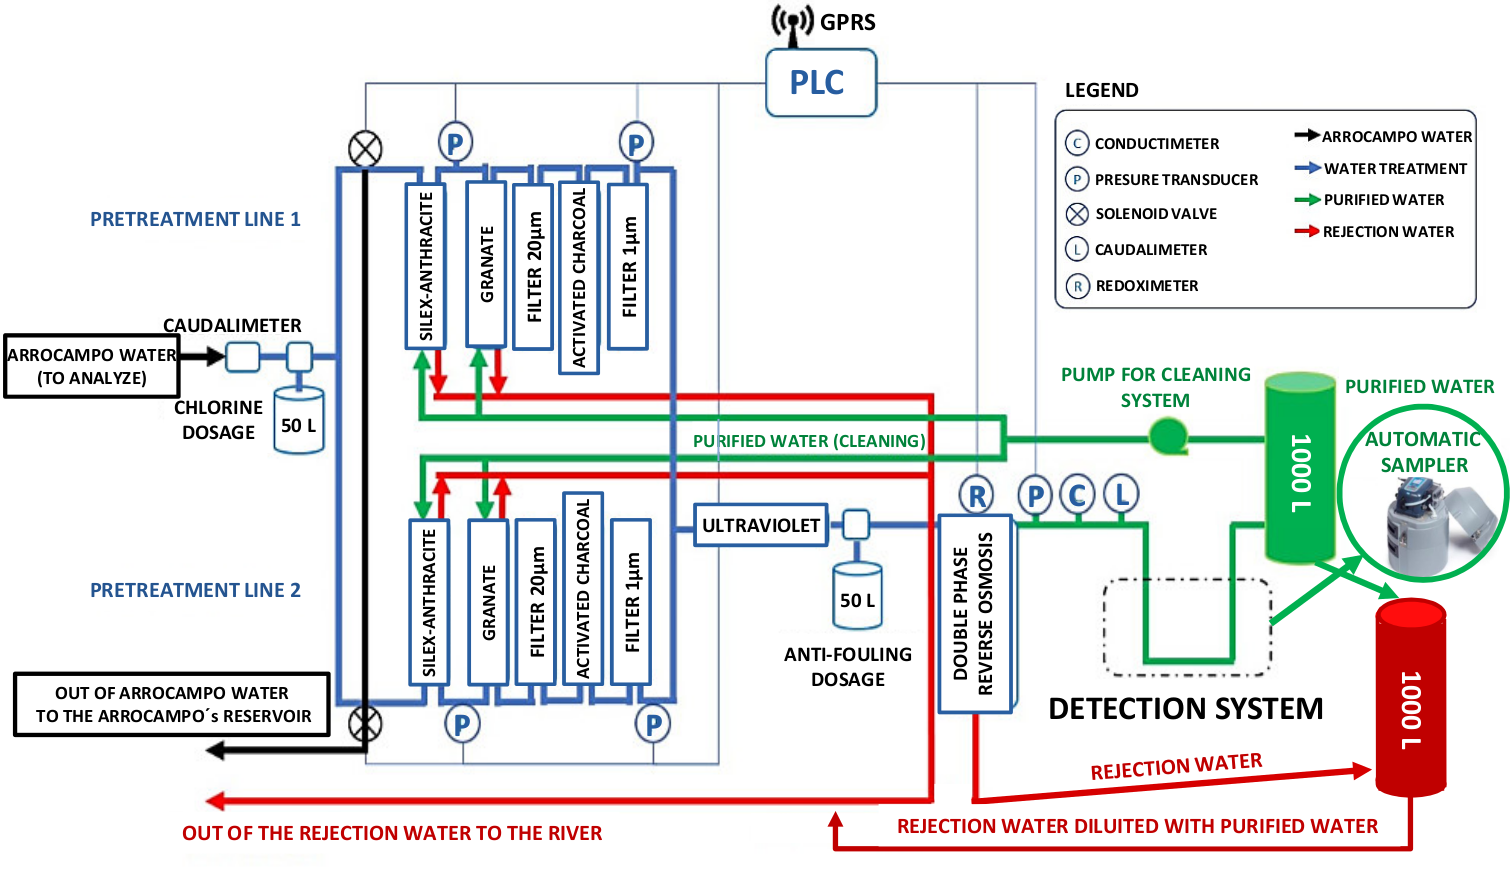
\includegraphics[width=14cm]{9Appendix/93UltraPureWaterSystem/SchemeUltraPureWaterSystem.png}
\caption{Scheme of the water purification system.\label{fig:SchemeUPWS}}
\end{figure}
The gross filtering stage made of silex-antracite and granate filters, the fine filtering stage consisting of a $20~\mu\meter$ filter and the super-fine filtering stage composed of a $1~\mu\meter$ filter of active carbon and UV lamps, are shown in Figure \ref{fig:UltraPureWaterStages}.
\begin{figure}
\centering
    \begin{subfigure}[b]{0.3\textwidth}
    \centering
    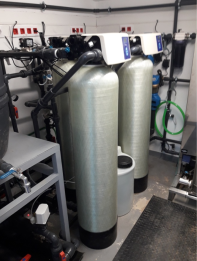
\includegraphics[width=\textwidth]{9Appendix/93UltraPureWaterSystem/GrossFiltering.png}  
    \caption{\label{subfig:GrossFiltering}}
    \end{subfigure}
    \hfill
    \begin{subfigure}[b]{0.3\textwidth}
    \centering
    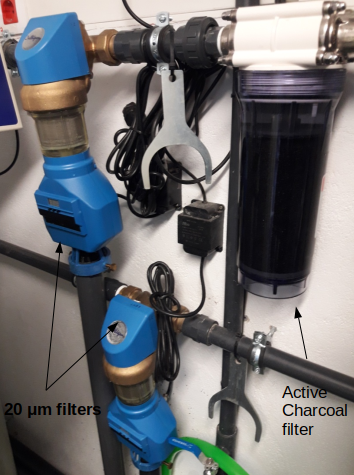
\includegraphics[width=\textwidth]{9Appendix/93UltraPureWaterSystem/FineFiltering.png}  
    \caption{\label{subfig:FineFiltering}}
    \end{subfigure}
    \hfill
    \begin{subfigure}[b]{0.3\textwidth}
    \centering
    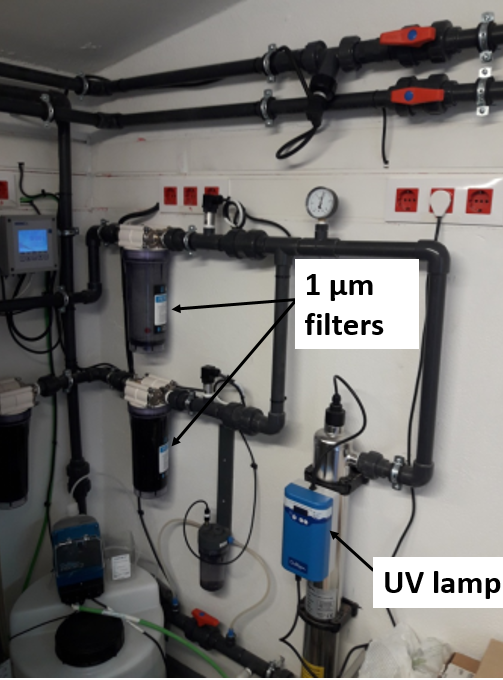
\includegraphics[width=\textwidth]{9Appendix/93UltraPureWaterSystem/SuperFineFiltering.png}  
    \caption{\label{subfig:SuperFineFiltering}}
    \end{subfigure}
 \caption{Different stages of filtration of the water purification system. a) The gross filtering stage. b) The fine filtering stage. c) The super-fine filtering stage.}
 \label{fig:UltraPureWaterStages}
\end{figure}
The double phase reverse osmosis and the containers in which pure and reject water are gathered after treatment are displayed in Figure \ref{fig:OsmosisContainers}.
\begin{figure}
\centering
    \begin{subfigure}[b]{0.5\textwidth}
    \centering
    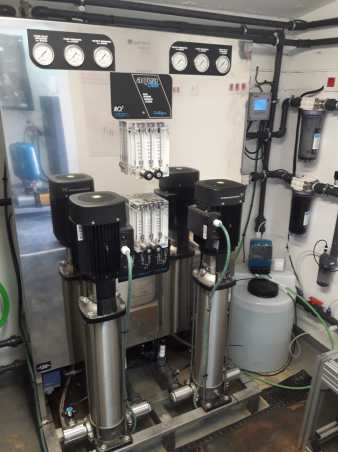
\includegraphics[width=\textwidth]{9Appendix/93UltraPureWaterSystem/Osmosi.png}  
    \caption{\label{subfig:Osmosi}}
    \end{subfigure}
    \hfill
    \begin{subfigure}[b]{0.8\textwidth}
    \centering
    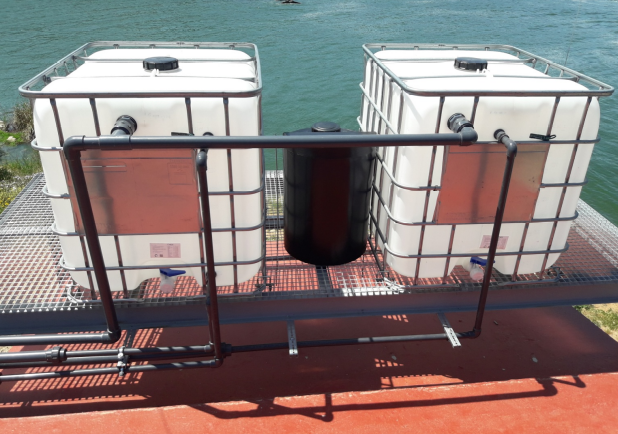
\includegraphics[width=\textwidth]{9Appendix/93UltraPureWaterSystem/Containers.png}  
    \caption{\label{subfig:Containers}}
    \end{subfigure}
 \caption{a) Doble phase reverse osmosis stage. b) Containers used to gather the output water of the water purification system.}
 \label{fig:OsmosisContainers}
\end{figure}
Two displays of the Siemens Programmable Logic Controller (PLC) that controls the water purification system is shown in Figure \ref{fig:Siemens}.
\begin{figure}
\centering
    \begin{subfigure}[b]{0.75\textwidth}
    \centering
    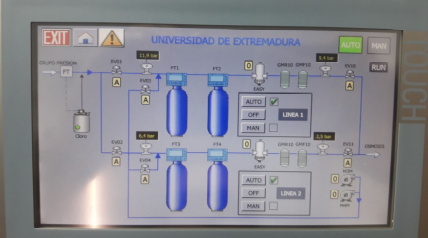
\includegraphics[width=\textwidth]{9Appendix/93UltraPureWaterSystem/Siemens1.png}  
    \caption{}
    \end{subfigure}
    \hfill
    \begin{subfigure}[b]{0.75\textwidth}
    \centering
    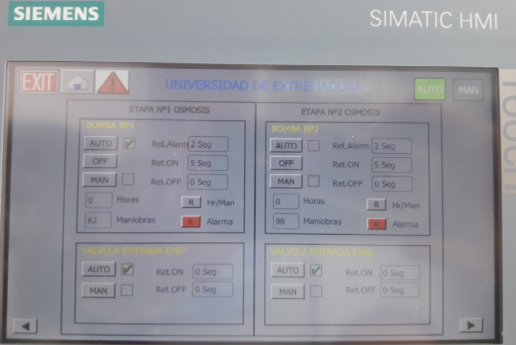
\includegraphics[width=\textwidth]{9Appendix/93UltraPureWaterSystem/Siemens2.png}  
    \caption{}
    \end{subfigure}
 \caption{Siemens PLC displays for the remote control of the water purification system.}
 \label{fig:Siemens}
\end{figure}
Finally, a picture of the whole water purification system is displayed in Figure \ref{fig:CompleteSystem}.
\begin{figure}[htbp]
\centering
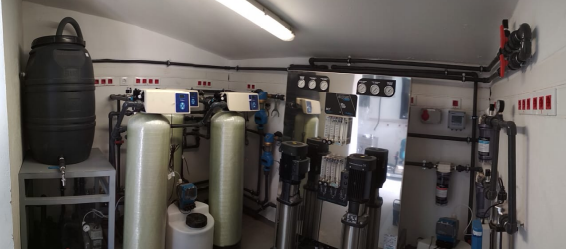
\includegraphics[scale=0.6]{9Appendix/93UltraPureWaterSystem/CompleteSystem.png}
\caption{Picture of the water purification system.\label{fig:CompleteSystem}}
\end{figure}
Samples of raw, rejected and pure water are shown in Figure \ref{fig:ThreeTypesOfWater}, where their difference in turbidity are distinguished.
\begin{figure}[htbp]
\centering
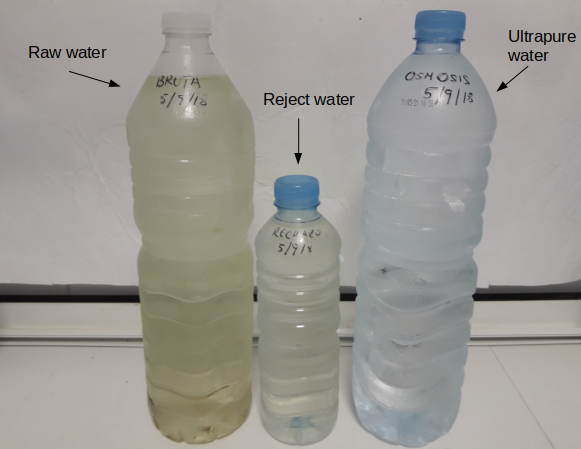
\includegraphics[scale=0.4]{9Appendix/93UltraPureWaterSystem/ThreeTypesOfWater.png}
\caption{Raw, reject and pure water obtained with the water purification system.\label{fig:ThreeTypesOfWater}}
\end{figure}